%!TEX root = ./WTG.tex
\marginnote{Beginn Vorlesung 21.04.2016}
Bislang haben wir gesehen, dass sich wichtige Fragen über Irrfahrten auf \enquote{elektrische Fragen} zurückführen lassen. Trefferwahrscheinlichkeiten entsprechen z.B. Spannungen, Durchquerungswahrscheinlichkeiten effektiven Kapazitäten usw. 
Durch Reduktion der Netzwerke lassen sich solche Größen auch berechnen. 

Heute wollen wir eine weitere Größe kennenlernen, die bei der Beantwortung von Fragen über Irrfahrten hilft.

\section{Energie}
\label{chap:Energie}
Sei zunächst $G = \enb{V,E,c}$ ein endliches Netzwerk.
\begin{definition}
	Sei $l^2\enb{V}$ die Menge aller Funktionen $F: V \to \RR$. $l^2(V)$ sei versehen mit dem üblichen Skalarprodukt 
	\begin{gather}
		\sprod{f,g} := \sum\limits_{v \in V} f(v)g(v), \Norm{f}^2 = \sprod{f,f}
	\end{gather}	
\end{definition}
\begin{definition}
	Sei $l^2(E)$ die Menge aller antisymmetrischen Funktionen 
	\begin{gather}
		\Theta = E \to \Real \text{ mit } \Theta(-e) = -\Theta(e)
	\end{gather}
	mit Skalarprodukt 
	\begin{gather}
		\sprod{\Theta,\Theta'} = \frac{1}{2}\sum\limits_{e \in E} \Theta(e) \Theta'(e) = \sum\limits_{e \in E_{1/2}} \Theta(e)\Theta'(e)
	\end{gather}
	wobei $E_{1/2}$ eine Teilmenge von $E$, die von jedem Paar $(e,-e), e \in E$ genau einen Vertreter enthält.
\end{definition}

\begin{definition}
	Sei $d:l^2(V) \to l^2(E)$ der \emph{Co-Rand-Operator}, definiert als
	\begin{gather}
		(df)(e) =  f(e^-) - f(e^+) \text{ wobei } e= (e^-,e^+)
	\end{gather}
	Weiter sei $d^*: l^2(E) \to l^2(V)$ der Rand Operator, definiert als
	\begin{gather}
		(d^*\Theta)(x) = \sum\limits_{e:e^-=x} \Theta(e)
	\end{gather}
\end{definition}
\begin{uebung}
	$\forall f \in l^2(V), \forall \Theta \in l^2_-(E)gilt$
	\begin{gather}
		\sprod{df,\Theta}_{l^2_-E} = \sprod{f,d^*\Theta}_{l^2(V)}
	\end{gather}
	Man kann Ohm und Kirchhoff mittels $d$ und $d^*$ elegant aufschreiben.
	\begin{itemize}
		\item Ohm: $dv = ir$, d.h. $\forall \ c \in E$ gilt $(dv)(e) = i(e) \cdot r(e)$.
		\item Kirchhoff: Für alle $x$, die nicht an einer Spannungsquelle liegen, gilt $(d^*i)(x)= 0$.
	\end{itemize}
\end{uebung}
Wir wollen nun Flüsse auf Netzwerken studieren. Ein Fluss $\Theta$ auf $G = (V,E,c)$ sei ein Element auf $l^2_-(E)$. Ein Fluss $\Theta$ heißt Fluss von $A$ nach $Z$, $A,Z \subseteq V, A \cap Z = \emptyset$, falls $g'H (d^*\Theta)(a) > 0, \forall a\in A , (d^*\Theta)(z)<0, \forall z \in Z$. Für alle $x \notin A\cup Z$ gilt $(d^*\Theta)(x) = 0$. Die \emph{Stärke} von $\Theta$ sei 
\begin{gather}
	S(\Theta) :=\sum\limits_{a \in A}(d^*\Theta)(a)
\end{gather}
$A$ heißt \emph{Quelle} und $Z$ heißt \emph{Senke}. Es gibt quellefreie  Flüsse. Vernünftige Flüsse wollen nichts verlieren:
\begin{lemma}
	Sei $G$ endlich, $A,Z \subseteq V, A \cap Z = \emptyset$. Dann gilt 
	\begin{align}
		S(\Theta) = -\sum\limits_{z \in Z}(d^*\Theta)(z)
	\end{align}
\end{lemma}
\begin{beweis}
	\begin{gather}
		\sum\limits_{a \in A} (d^*\Theta)(a) + \sum\limits_{z \in Z} (d^*\Theta)(z) = \sum\limits_{x \in V}(d^*\Theta)(x) \cdot 1 = \sprod{d^*\Theta,\mathds{1}} = \sprod{\Theta,d \mathds{1}} = 0. \marginnote{$d \mathds{1} = 0$}
	\end{gather}
\end{beweis}

\begin{lemma}
	Sei $G$ endlich, $A,Z \subseteq V, A\cap Z = \emptyset$ und $\Theta$ ein Fluss von $A$ nahc $Z$. Sei $f \in l^2(V)$ mit $f|_A \equiv \alpha, f|_Z = \zeta$. Dann gilt
	\begin{gather}
		\sprod{\Theta,df} = (\alpha - \zeta) S(\Theta).
	\end{gather}
\end{lemma}
\begin{beweis}
	\begin{align}
		\sprod{\Theta,df} &= \sprod{d^*\Theta,f} = \sum\limits_{x \in V} (d*\Theta)(x)f(x) \\
			&= \alpha\sum\limits_{x\in A} (d^* \Theta)(x) + \sum\limits_{x \notin A \cup Z} (d^*\Theta)(x)f(x) + \zeta\sum\limits_{x\in Z} (d^*\Theta)(x) \\
			&= \alpha S(\Theta) + 0 - \zeta S(\Theta)  = (\alpha - \zeta) S(\Theta)
	\end{align}
\end{beweis}
Idee aus der Physik: An einem Widerstand der Stärke $v$ wird eine Arbeit der Stärke $s^2v$ geleistet. Wir übertragen das auf Flüsse auf Netzwerken:
\begin{definition}
	Für einen beliebigen Vektrorraum $H$ mit Skalarprodukt $<\cdot,\cdot>$ definiere für $f,g,h \in H$
	\begin{align}
		\sprod{f,g}_h = \sprod{fh,g} = \sprod{f,gh} && \Norm{f}^2_v = \sprod{f,f}.
	\end{align}
\end{definition}
Für $\Theta \in l^2_-(E)$ sei $\mathcal{E}(\Theta) = \Norm{\Theta}^2_v$ die Energie von $\Theta$. Insbesondere ist für einen Stromfluss $i$. $\mathcal{E}(i) = \Norm{i}^2_v = \sprod{i,i\cdot v}  =\sprod{i, dv}$ nach Ohm.

\begin{uebung}
	Für $A\cap Z = \emptyset$ definiere $C(A \leftrightarrow Z)$ als $C(a \leftrightarrow Z)$, wenn man alle $x \in A$ zu $a$ identifiziert nun entsprechend $R(A \leftrightarrow Z) = \frac{1}{C(A \leftrightarrow Z)}$. Man zeige, dass dann für
	\begin{align} 
		v|_A \equiv \text{const.} = v_A && v|_Z \equiv \text{const.} = v_Z \\ 
	\end{align}
	\begin{align}
		v_A - v_Z = \mathcal{I}_{AZ}R(A \leftrightarrow Z) \text{ gilt, wobei } \mathcal{I}_{AZ} = \sum\limits_{a \in A}\sum\limits_{x \sim a}i(a,x)
	\end{align}
	
	Damit lässt sich die Energie für einen Einheitstrom mit $v|_A \equiv \alpha, v|_Z \equiv \xi$ berechnen durch 
	\begin{align}
		\mathcal{E}(i) = \enb{\alpha - \xi} S(i) = \alpha - \xi = \mathcal{R}(A \leftrightarrow Z)
	\end{align}
\end{uebung}

Sei $X^l = \mathds{1}_{\set{e}} - \mathds{1}_{\set{-e}}$, $X^l \in l^2_-(E)$. Dann gilt für alle $\Theta \in l^2_-(E):$
\begin{gather}
	\sprod{\Theta,\chi^e}_r = \Theta(e)r(e)
\end{gather}
Somit 
\begin{gather}
	\sprod[\Big]{\sum\limits_{e \cdot e^ = x} c(e)\chi^e,\Theta} = \sum\limits_{e \cdot e^-}\sprod[\big]{c\enbrace[\big]{e\chi^e,\Theta(e)}} = \sum\limits_{e^-=x} \Theta(e) = (d^*\Theta)(x).
\end{gather}
Wenn an $x$ keine Spannung anliegt, sagt Kirchhoff
\begin{gather}
	\sprod[\Big]{\sum\limits_{e \cdot e^- = x} c(e)\chi^e,\Theta} = 0
\end{gather}
Die kirchhoffsche Maschenregel lässt sich schreiben als 
\begin{gather}
	\sprod[\Big]{\sum\limits_{k=1}^{n}\chi^{e_k},i} = 0 \text{, für einen gerichteten Kreis } e_1, \dots, r_n
\end{gather}
Definiere
\begin{align}
	\bigstar &= \Span \set{\Theta \in l^2_- \in E \given \Theta = \sum\limits_{e \cdot e^- = x}c(e)\chi^e} \\
	\bigcirc &= \Span \set{\Theta \in l^2_-(E) \given \Theta = \sum\limits_{k=1}^{e_n}\chi^{e_k}} \text{, für einen gerichteten Kreis} e_1, \dots e_n
\end{align}

\begin{uebung}
	$\bigstar$ und $\bigcirc$ sind bezüglich $\sprod{\cdot,\cdot}_r$ auf $E$ orthogonal
	\begin{gather}
		\bigstar \oplus \bigcirc = l^2_-(E)
	\end{gather}
Das Kirchhoffsche Maschengesetz sagt nun, dass jeder Stromfluss $i$ orthogonal zu $\bigcirc$, also in $\bigstar$ ist (bezüglich $\sprod{\cdot,\cdot}_r$). Ist $\Theta \in l^2_-(E)$ und $i$ ein Stromfluss mit $d^*\Theta = d^*i$, dann gilt $d^*(\Theta - i) = d^*\Theta - d^*i = 0$, d.h. $\Theta -i$ ist quellenfrei. Somit folgt aus (2), dass $\Theta - i \in \bigcirc$. Also hat man $\Theta = i + \enb{\Theta-i}$ als orthogonale Zerlegung. 
\end{uebung}
Es folgt aus der orthogonalen Zerlegung von $\Theta$ in $i$ und $\Theta - i$, dass $\Norm{\Theta}^2_r = \Norm{i}^2_r + \Norm{\Theta - i}^2_r$. Dies ergibt sofort folgendes Satz:
\begin{satz}[Thompsonsches Prinzip]
	\label{satz:Tompson}
	Sei $G$ endlich, $A,Z \subseteq V, A \cap Z = \emptyset.$ Sei $\Theta$ ein Fluss von $A$ nach $Z$ und $i$ in der Stromfluss von $A$ nach $Z$, mit $(d^*\Theta) = (d^2i)$. Dann gilt $\mathcal{E}(\Theta) \geq \mathcal(i)$
\end{satz}
\begin{beweis}
	Folgt, da $\mathcal{E}(\Theta) = \Norm{\Theta}^2_r$
\end{beweis}

\begin{satz}[Rayleighsches Prinzip]
	\label{satz:Rayleigh}
	Sei $G$ endlich, $A,Z \subseteq V, A \cap Z = \emptyset$. Seien $c,c' : E \to \RR$ Leitfähigkeiten und $c \leq c'$. Dann gilt
	\begin{align}
		\mathcal{C}_c\enb{A \leftrightarrow Z} \leq \mathcal{C}_{c'} \enb{A \leftrightarrow Z}
	\end{align}
\end{satz}
\begin{beweis}
	Es gilt
	\begin{gather}
		\mathcal{E}(i_c) =  R_c(A \leftrightarrow Z) = \frac{1}{\leit{A \leftrightarrow Z}}
	\end{gather}
	und 
	\begin{gather}
		\mathcal{E}_c(i_c) = ||i_c||^2_r = ||i_c||^2_{\frac{1}{c}} =\geq ||i_c||^2_{\frac{1}{c'}} \geq \mathcal{E}_{c'}(i_c) \geq \mathcal{E}_{c'}(i_{c}).
	\end{gather}
	Kehrwert Bilden ergibt $\mathcal{C}_c(A \leftrightarrow Z) \leq \mathcal{C}_{c'} (A \leftrightarrow Z)$
\end{beweis}

\marginnote{Vorlesungsbeginn 25.04.2016}
\section{Transienz \& Rekurrenz}
\label{chap:TransienzUndRekurrenz}

Wir haben gesehen: Begriffe wie \enquote{effektive Kapazität}, \enquote{effektiver Widerstand}, \enquote{Energie}, \enquote{Spannung} helfen, um das Verhalten von Irrfahrten auf Graphen besser zu verstehen. Zum Beispiel entsprechen Spannungen Treffwahrscheinlichkeiten effektive Widerstände bzw. Kapazitäten entsprechen Durchgangswahrscheinlichkeiten, Energie ist so etwas wie effektive Widerstände.

Bislang haben wir einiges erst auf endlichen Graphen definiert, dieses Setup ist für Fragen der Rekkurenz und Transienz jedoch zu klein. Sei nun $G$ unendlich. Wir definieren wieder

\begin{gather}
	l^2(V) = \set{f:V \to \Real: \sum\limits_{v\in V} f^2(v)<\infty } \text{mit Skalarprodukt } \sprod{f,g} = \sum\limits_{v \in V} f(v)g(v),  \Norm{f}^2 = \sprod{f,f}
\end{gather}
und mit $e = \enb{e^+,e^-}, -e = \enb{e^-,e^+}$
\begin{gather}
	l^2_-(E) = \set{\Theta:E \to \Real: \Theta(-e) = -\Theta(e), \sum \Theta^2(e)r(e) < \infty} \\
	 \text{mit Skalarprodukt } \sprod{\Theta, \Theta'}_r = \sum\limits_{e \in E_{1/2}} \Theta(e)\Theta'(e)r(e) \text{ und Energie } \mathcal{E}(\Theta) = \Norm{\Theta}^2_r
\end{gather}

Man kann dann den Co-Randoperator $(df)(e)= d(e^-) - f(e^+)$ definieren, den Randoperator $(d^*\Theta)(x) = \sum\limits_{x = c^-}\Theta(e)$ und man erhält wieder deren Dualität. Man kann sich vergewissern, dass sich so das gesamte Kapitel \ref{chap:Energie} auf die unendliche Situation verallgemeinern lässt. Wir wollen nun Flüsse aus einem $a \in V$ nach unendlich betrachten, d.h. $\Theta$ ist von der Form $d^*\Theta(x) := \alpha \mathds{1}_{\set{a}}(x)$. 

Wir wollen die Frage der Transienz in Beziehung zur Existenz solcher Flüsse setzen.

\begin{satz}[Lyons]
	Wenn $G$ ein abzählbares, zusammenhängendes Netzwerk ist, dann ist die Irrfahrt auf $G$ genau dann transient, wenn es einen Fluss endlicher Energie von einem $a \in V$ nach $\infty$ gibt.
\end{satz}
\begin{beweis}
	Sei $G_n  \subseteq G$ endlich, $G_n \uparrow G$. Die Punkte in $V \backslash V_n$ kleben wir wieder summen zu $z_n$, behalten Doppelkanten und werfen Schlaufen weg. Das resultierende Netzwerk sei $G^w_n$, sei o.E. $a \in G_n$. 
	
	Es gilt $R(a \leftrightarrow \infty) = \lim R(a \leftrightarrow z_n)$.
	Nun ist einerseits $R(a \leftrightarrow z_n) = \frac{1}{\leit{a \leftrightarrow z_n}} \sim \frac{1}{\prop{\tau^+_a < \tau_{z_n}}}$, d.h. 
	\begin{equation}
		\lim R(a \leftrightarrow z_n) < \infty \Leftrightarrow \lim\limits_{n \to \infty} \prop{a \to z_n} < 0. \marginnote{Transienz}
	\end{equation}
	Auf der anderen Seite ist $\lim R(a \leftrightarrow z_n) = \lim \mathcal{E}(i_n)$ für einen Einheitsstrom $i_n$ von $a$ nach $z_n$. Das heißt Transienz der Irrfahrt ist äquivalent zur Endlichkeit von $\lim \mathcal{E}(i_n)$. Sei nun $\Theta$ irgendein Einheitsfluss endlicher Energie von $a$ nach $\infty$. Sei $in$ der Einheitsstrom-Fluss von $a$ nach $z_n$, $\Theta_n = \Theta|_{G^W_n}$. Dann gilt nach Thompson (\ref{satz:Tompson})
	\begin{align}
		\mathcal{E}(i_n) \leq \mathcal{E}(\Theta_n) = \mathcal{E}(\Theta) < \infty \text{, für alle } n
	\end{align}
	$\Rightarrow \lim \mathcal{E}(i_n) < \infty \Rightarrow$ Die Irrfahrt ist transient. \\
	
	Sei nun die Irrfahrt transient. Wir wollen nun einen Fluss von $a$ nach $\infty$ endlicher Energie basteln, Kandidat: $\lim i_n.$ Nach der Vorüberlegung gilt;
	\begin{align}
		\exists N > 0: \lim \mathcal{E}(i_n) \leq N < \infty, (\mathcal{E}(i_n)\leq N \forall n)
	\end{align}
	Sei nun 
	\begin{align}
		Y_n(x) &= \text{Anzahl der Besuche der Irrfahrt bei Start in $a$ in $x$ vor Verlassen von } G_n \\
		Y(x) &= \text{Anzahl der Besuche der Irrfahrt bei Start in $a$ in $x$} 
	\end{align}
	Dann gilt mit der monotonen Konvergenz:
	\begin{align}
		\EWE{Y(x)} = \EWE{\lim Y_n(x)} = \lim\limits_{n \to \infty} \EWE{Y_n(x)} = \lim\limits_{n \to \infty} \pi(x) v_n(x) = \pi(x)v(x) \marginnote{$v_n(x)$ Spannung von $x$ in $G_n$}
	\end{align}
	Da die Irrfahrt transient ist, ist die linke Seite endlich, also existiert $\lim v_n(x) = v(x)$. Also ist
	\begin{align}
		\Gamma := c (dv) = \lim\limits_{n\to\infty} c (dv_n) = \lim\limits_{n\to\infty} i_n
	\end{align}
	der Strom auf $G$.

	Die ist ein Stromfluss endlicher Energie nach der folgenden Übung.
\end{beweis}

\begin{uebung}
	$G$ abzählbar, $(\Theta_n)_n \subset l^2_-(E): \mathcal{E}(\Theta_n) \leq M < \infty$ für ein $M$ und $\Theta_n(e) \to \Theta(e)$. Dann ist $\Theta$ antisymmetrisch und $\mathcal{E}(\Theta) \leq \liminf \mathcal{E}(\Theta_n)$ und es gilt $ \forall x: (d^*\Theta_n)(x) \to (d^*\Theta)(x)$
\end{uebung}

Allgemeiner gilt (ohne Beweis)

	\begin{satz}
		Sei $G$ transient und zusammenhängend, $G_n \uparrow G$, $G_n$ endlich. $G_n^W$ kostruiert wie immer und $i_n$ der Einheitsstrom in $G^W_n$ von einem $a$ nach $z_n$ Dann:
		
		$i_n$ konvergiert punkt-(d.h. Kanten-) weise gegen ein $i$, der Einheitsstromfluss von $a$ nach $\infty$.

	Sind $v_n$ die zugehörigen Spannungen in $G^W_n$ mit $v(z_n) = 0,$ gilt $v  = \lim v_n$ existiert.

	Es gilt:
	\begin{align}
		dv = ir && v(0) = \mathcal{E} = R(a \leftrightarrow \infty) && \forall x: \frac{v(x)}{v(0)} = \prop{\tau_a < \infty}
	\end{align}
	Weiter sei $\mathcal{G}(a,x) := \pi(x)v(x) = \EW{\text{Treffer von }x}.$ Schließlich 
	\begin{equation}
		i(l) = \EW{\text{Anzahl signierte Überquerungen von}e} 
	\end{equation}

\end{satz}
Wie findet man nun heraus ob es einen Fluss endlicher Energie von einem $a\in V$ nach $\infty$ gibt? Für die erste Methode benötigen wir die folgende Definition
\begin{definition}
	$\pi \subseteq E$ heißt \emph{Cut-Set} zwischen $a$ und $\infty$, wenn jeder Pfad $\gamma$ von $a$ nach $\infty$ die Ungleichheit $\gamma \cap \pi \neq \emptyset$ erfüllt.
\end{definition}

\begin{satz}[Nash-Williams]
	\label{satz:Nash-Williams}
	Sei $(\pi_n)$ eine Folge paarweise disjunkter Cut-Sets, die $a$ von $\infty$ trennt. Dann gilt 
	\begin{align}
		R(a \leftrightarrow \infty) \geq \sum\limits_{n = 1}^{\infty}\enb{\sum\limits_{e \in \pi_n} c(e)}^{-1}
	\end{align}
\end{satz}

\begin{bemerkung}
	\begin{enumerate}[a)]
		\item Ist für eine Folge von $\Pi_n$ wie Satz \ref{satz:Nash-Williams} die rechte Seite unendlich, so ist die Irrfahrt rekurrent
		\item Intuitiv sollte die Aussage des Satzes \ref{satz:Nash-Williams} klar sein, denn jedes $Pi_n$ hat einen Widerstand $ \geq \enb{\sum\limits_{l\in \Pi_n} c(e)}^{-1}$
	\end{enumerate}
\end{bemerkung}
\begin{beweis}
	$\Theta$ sei ein Einheitsfluss von $a$ nach $\infty$. Es gilt:
	\begin{align}
		\sum\limits_{e \in \Pi_n} \Theta^2(e) r(e) \sum\limits_{e \in \Pi_n} c(e) \geq \enb{\sum\limits_{e \in \Pi_n}\abs{\Theta(e)} \sqrt{r(e)}\sqrt{c(e)}}^2 = \enb{\sum\limits_{e \in \Pi_n}\abs{\Theta(e)}}^2 \geq \enb{\sum\limits_{e \in F_n}\abs{\Theta(e)} }^2
	\end{align}
	wobei $k_n$ (kommt noch) die Menge aller Kanten ist, die \underline{nicht} von $a$ getrennt werden durch $\Pi_n$, und $F_n$ die Menge aller Kanten $c = (e^-,e^+)$ mit $e^- \in k_n$, aber $e^+ \notin k_n$. Es ist klar, dass $F_n \leq \Pi_n$.
	
	Nun ist 
	\begin{gather}
		\sum\limits_{r \in F_n} \abs{\Theta_i(e)} \geq \sum\limits_{e \in F_n} \Theta(e) = \sum\limits_{x \in k_n} (d^*\Theta)(x) = (d^*\Theta)(a) = 1 \\
		\Rightarrow \sum\limits_{e \in \Pi_n} \Theta^2(e)r(e) \geq \frac{1}{\sum\limits_{c \in \Pi_n}c(e)}.
	\end{gather}
	Also 
	\begin{align}
		R (a \leftrightarrow \infty) = \mathcal{E}(i) \geq \sum\limits_{n \geq 1}\sum\limits_{e\in \Pi_n} \Theta^2(e)r(e) \geq \sum\limits_{n \geq 1} \enb{\sum\limits_{e \in\Pi} c(e)}
	\end{align}
	
	
\end{beweis}

Für einen Transienz--Beweis hilft Nash-Williams zunächst nicht. Hier versuchen wir die zufällige Pfadwahl. Dazu sei $\p$ eine Wahrscheinlichkeit auf der Menge der Pfade von $a$ nach $\infty$. So ein Pfad $(e_n)$ entspricht einem Einheitsfluss
\begin{gather}
	\psi^{(e_n)} (e) := \sum\limits_{n \geq 1} \chi^{e_n} = \sum\limits_{n \geq 1} \mathds{1}_{\set{e_n}}- \mathds{1}_{\set{-e_n}}
\end{gather}
Da alle $(e_n)$ in $a$ starten, ist die Erwartung dieses Einheitsfluss von $a \to \infty$  
\begin{align}
	\Theta = \EW{\psi} = \sum\limits_{n \geq 1}\prop{e_n} - \prop{-e_n}
\end{align}
Von einem solchen $\Theta$ möchte man die Energie beschränken. 

\marginnote{Beginn Vorlesung vom 28.04}
Wir haben nun elektrische Größen in Beziehung zu Fragen von Rekurrenz und Transienz in Netzwerken gesetzt. Insbesondere gilt: Ist $\mathcal{R}(a \leftrightarrow \infty)  = \infty $, so ist die Irrfahrt rekurrent. Kann man umgekehrt einen Fluss $\Theta$ endlicher Energie von $a$ nach $\infty$ finden, dann ist $\mathcal{R}(a \leftrightarrow \infty)< \infty$ und die Irrfahrt ist transient. Das erste Kriterium lässt sich mit Hilfe des Satzes von Nash-Williams (\ref{satz:Nash-Williams}) überprüfen: Umgekehrt kann man versuchen, einen Fluss zu konstruieren, der möglichst gut an $(c(e))$ angepasst ist. Man kann z.B. eine Menge von Pfaden $\set{(e_n)_n}$ hernehmen, die von $a$ nach $\infty$ laufen und darauf ein Wahrscheinlichkeitsmaß $\p$. Zu einem Pfad $(e_n)$ gehört ein Einheitsfluss \todo{Stimmt das so?(von hand verbessert)}
\begin{align}
	\psi^{(e_n)}_{(e)} = \sum\limits_{n \geq 1} \mathds{1}_{\set{e_n = e}} - \mathds{1}_{\set{e_n = -e}}
\end{align}
Die Erwartung dieses Einheitsflusses ist
\begin{gather}
	\Theta(e) = \sum\limits_{n \geq 1} \prop{e_n = e} - \prop{e_n = -e} \tag{$*$}\label{eqn:4-1}
\end{gather}
Wählt man $\p$ so, dass Kanten hoher Leitfähigkeit oft benutzt, und Kanten niedriger Leitfähigkeit wenig, kann man hoffen einen Fluss endlicher Energie von $a \to \infty$ zu konstruieren. Ein Beispiel ist der folgende Satz

\begin{satz}[Polyò]
	Die Irrfahrt auf $\ZZ^d$ ist rekurrent für $d\leq 2$ und transient für $d \geq 3$.
\end{satz}
\begin{beweis}
	Für $d=1,2$ verwenden wir das Kriterium von Nash-Williams (\ref{satz:Nash-Williams}).
	
	\begin{figure}
		\centering
		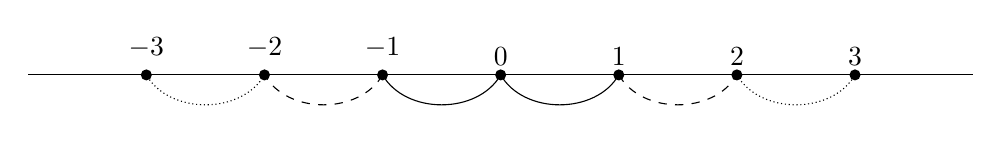
\begin{tikzpicture}[scale=1.5, every node/.style=fill,circle,minimum size=4pt,inner sep=0pt]
			\draw (0,0) to (8,0);
			\foreach \x in {1,...,7}
			{
				\node[label=above:{\pgfmathparse{\x - 4}% Evaluate the expression
					\pgfmathprintnumber[    % Print the result
					fixed,
					fixed zerofill,
					precision=0
					]{\pgfmathresult}}] at (\x,0) {};
			}
		
			\draw[bend angle=60,bend right] (4 ,0) to (5, 0);
			\draw[bend angle=60,bend left] (4,0) to (3, 0);
			
			\draw[bend angle=60,bend right, dashed] (4 + 1,0) to (5 + 1, 0);
			\draw[bend angle=60,bend left, dashed] (4 - 1,0) to (3 - 1, 0);
			
			\draw[bend angle=60,bend right, densely dotted] (4 + 2,0) to (5 + 2, 0);
			\draw[bend angle=60,bend left, densely dotted] (4 - 2,0) to (3 - 2, 0);
			
		\end{tikzpicture}
		\caption{Cutsets in $d=1$}
		\label{fig:7}
	\end{figure}
	Betrachten wir die Cutsets $\Pi_n$ wie in \autoref{fig:7}, so gilt 
	\begin{gather}
		(a \leftrightarrow \infty) \leq \sum\limits_{n \geq 1} \enb{\sum c(e) }^{-1} = \sum\limits_{n \geq 1 } \frac{1}{2} = \infty
	\end{gather}
	
	Sei $n = 2$, dann
	
	\begin{gather}
		\Pi_n = \set{e = (x,y) \given x \in Q_n, y \in Q_{n+1}}
	\end{gather}
	$Q_n$ sei der Quader der Kantenlänge $n$ \todo[inline]{missing figure}
	$\abs{\Pi_n} = 8n + 4$. Damit erhält man 
	\begin{gather}
		R(a\leftrightarrow \infty) \geq \sum\limits_{n \geq 1} \enb{\sum\limits_{c \in \Pi} 1}^{-1} = \sum\limits_{n \geq 1} \frac{1}{8n + 4} = \infty
	\end{gather}
	Nach Rayleigh (\ref{satz:Rayleigh}) genügt es für die Transienz den Fall $d=3$ zu betrachten. 
	
	\underline{Idee:} Wähle alle Pfade, die \enquote{direkt} von $0$ nach $\infty$ laufen \enquote{mit gleicher Wahrscheinlichkeit}.
	
	Wir wählen einen Punkt $s \in S^2$ nach dem Haarschen Maß. Konstruiere eine Gerade durch $\overrightarrow{0s}$. Wähle zu jeden $\overrightarrow{0s}$ einen Pfad in $\ZZ^3$, der nach $\infty$ läuft und \enquote{direkt} an $\overrightarrow{0s}$ liegt (Es gibt einen solchen Pfad, der Abstand $\leq 4$ hat). \todo{figuuuuure}
	Das gibt eine Menge von Pfaden $\set{(e_n)}$ und hierauf habe ich ein Wahrscheinlichkeit die durch das Haar--Maß induziert wird. Wir wollen für das wie in \eqref{eqn:4-1} konstruierte $\Theta$ $\mathcal{E}(\Theta)$ berechnen.
	\begin{align}
		\mathcal{E}(\Theta) &= \sum\limits_{e} \Theta^2(e) r(e) = \sum\limits_{e}\Theta^2(e) \leq \sum\limits_{e} \prop{e_n=e}[2] \\
							&= \sum\limits_{n=1}^{\infty} \sum\limits_{e\colon d(0,e^+) = n}\prop{e_n = e}[2] \\
							&= \sum\limits_{n = 1}^{\infty}Cn^2\frac{c'}{n^4} = const \sum\limits_{n \geq} \frac{1}{n^2} < \infty \marginnote{Es gibt $Cn^2$ viele Kanten mit $d(0,e^+) = n$} 
	\end{align}
	
	Die Wahrscheinlichkeit eine Kante zu benutzen ist nach oben beschränkt durch $\frac{c'}{n^2}$, weil durch die Wahl von $s$ alle kanten im Bastand \enquote{ungefähr gleich} häufig getroffen werden.
	
\end{beweis}

\chapter{Spezielle Netzwerke}
\label{chap:SpezielleNetzwerke}
\section{Flüsse, Cutsets und Ford Fulkerson}
Gegeben sei irgendein Netzwerk $G = (V,R,c).$ Sei $a,(z) \in V$ oder $z = \infty$. Gibt es einen Fluss $\Theta$ von $a$ nach $z$, dergestalt
\begin{gather}
	\abs{\Theta(e)} \leq c(e)  \text{ für alle } e?
\end{gather}
Zum Beispiel gilt für den Einheitsstromfluss von $a$ nach $z$ mit Spannungen $v$, dass 
\begin{align}
	\abs{i(e)} = \abs{c(e) dv(e)} \leq c(e)v(a)
\end{align}
Somit ist $\frac{i}{v(a)}$ ein Fluss von $a$ nach $z$, mit $\frac{\abs{i(e)}}{v(a)} \leq c(e)$. Solche Flüsse wollen wir zulässig nennen.
\todo[inline]{missing figure. böum}
Die erste Frage ist: Was ist die maximale Flussstärke eines zulässigen Flusses von $A$ nach $Z$ mit $A \cap Z = \emptyset$?
\todo[inline]{uuuuuund noch eine Zeichnung}
Es ist intuitiv zu erwarten, dass ein Fluss nicht stärker sein kann, als die Summe der Leitfähigkeiten der Gewichte in einem Cutset. \marginnote{\enquote{Katze!}} Das erstaunliche ist, dass man auf diese Weise tatsächlich die maximale Flussstärke ermitteln kann. Es gilt

\begin{satz}[Ford Fulkersen, Max--Flow--Min--Cut--Theorem]
	Sei $G = (V,E,c)$ ein ungerichteter, endlicher Graph. Sei $A,Z \subset V, A \cap Z = \emptyset$. Dann gilt für zulässige Flüsse $\Theta$ von $A$ nach $Z$
	\begin{align}
		\max\limits_{\Theta \text{ zulässig}} S(\Theta) = \min \set{\sum\limits_{e \in \Pi}c(e) \given \Pi \text{ ist ein $A$--$Z$ Cut--Set}}
	\end{align}
\end{satz}
Wir beweisen allgemeiner eine Version für gerichtete Graphen
\begin{beweis}
	Dazu sei $G = (V,E,c), E \subseteq V \times V$. Dabei ist $c(e) = c(-e)$ nicht mehr notwendigerweise erfüllt. Sei
	\begin{align}
		\phi (x,e) = \mathds{1}_{\set{x = e^-}}- \mathds{1}_{\set{x = e^+}}
	\end{align}
	die Kanten-Knoten-Inzidenz-Funktion.

\end{beweis}

\begin{definition}
	$\Theta\colon E \to \RR^+$ heißt Fluss von $A$ nach $Z$ mit $A \cap Z = \emptyset$, wenn gilt
	\begin{align}
		x \in A &\Rightarrow \sum\limits_{e} \phi(x,e) \Theta(e) > 0 \\
		x \in Z &\Rightarrow \sum\limits_{e} \phi(x,e) \Theta(e) < 0 \\
		x \notin A \cup Z &\Rightarrow \sum\limits_{e} \phi(x,e) \Theta(e) = 0
	\end{align}
	$A$ heißt \emph{Quelle}, $Z$ heißt \emph{Senke} von $\Theta$. $\Theta$ heißt \emph{zulässig}, wenn $\Theta(e) \leq c(e)$ für alle $e \in E$. Die \emph{Flussstärke} $S$ ist definiert durch
	\begin{align}
		S(\Theta):= \sum\limits_{x \in A} \sum\limits_{e \in E} \phi(x,e) \Theta(e)
	\end{align}
\end{definition}
	
\begin{satz}
	\label{satz:5-3}
	$G = (V,E,c)$ gerichtetes, endliches Netzwerk. Dann gilt für zulässiger Flüsse $\Theta$ von $A$ nach $Z$ mit $\abs{\Theta(e)}  \leq c(e), \forall e$:
	\begin{align}
		\max\limits_{\Theta \text{ zulässig}}\set{S(\Theta)}  = \min\set{\sum\limits_{e \in \Pi}c(e) \given \Pi \text{ ist ein $A$--$Z$ Cutset}}
	\end{align}
\end{satz}
\begin{beweis}
	Das Maximum existiert und wird angenommen. Die Menge aller Flüsse $T := \set{\Theta \colon E \to \RR^+ \given \Theta \text{ ist zulässiger $A$--$Z$--Fluss}}\subseteq \RR_+^{\abs{E}}$. Aus der Zulässigkeitsbedingung folgt $\Theta(e) \leq c(e), \forall e$. Damit ist die Menge aller zulässigen Flüsse abgeschlossen und beschränkt in $\Real^{\abs{E}}$, also kompakt. $S$ ist stetig in $\Theta$, somit wird das Maximum sowie das Minimum auf $T$ angenommen. 
	
	Sei $\Theta$ maximierend, sei $\Pi$ ein $A$--$Z$--Cutset. Dann ist $A'$ die Menge der Vertizes, die nicht durch \todo{malen malen malen} $\Pi$ von $A$ getrennt werden. Insbesondere ist $A \subseteq A'$. Dann gilt
	\begin{align}
		S(\Theta) = \sum\limits_{x \in A}\sum\limits_{c \in E} \phi(x,e) \Theta(e) = \sum\limits_{x \in A'} \sum\limits_{c \in E} \phi(x,e) \Theta(e)
	\end{align}
	da $A' \supseteq A$ und $\sum\limits_{e} \phi (x,e) \Theta(e) = 0$ für $x \in A' \backslash A.$
	\begin{align}
		\dots = \sum\limits_{c \in E}\Theta(e)\sum\limits_{x\in A'}\phi(x,e) \leq \sum\limits_{e \in \Pi} \Theta(e) \leq \sum\limits_{e \in \Pi} c(e)
	\end{align}
	Nun ist
	\begin{align}
		\sum\limits_{x \in A'} = 
			\begin{cases}
			0, & \text{wenn } e = (a',a'') \text{ mit } a',a'' \in A \text{ oder } a',a'' \notin A' \\
			1, & \text{wenn } c = (a',y), a' \in A', y\notin A'\\
			-1, & \text{wenn } e= (y,a'), a' \in A', y \notin A'
			\end{cases}
	\end{align}
	Für die andere Richtung definieren wir für $\Theta$, dass $x_0,x_1, \dots , x_k$ ein vergrößerbarer Pfad ist, wenn $x_0 \in A$ und für alle $i = 1,\dots,k$ gilt, dass entweder
	\begin{align}
		e = (x_{i-1}x_i) \in E \text{ und } \Theta(e) < c(e) \\
		e' = (x_i,x_{i-1}) \in E \text{ und } \Theta'(e) > 0.
	\end{align}
	
	Sei $B= \set{y \in V \given \exists \text{ vergrößerbarer Pfad von einem $x \in A$ nach $y$}}$, mit Nebenbedingung $A\subseteq B$.
	
	\underline{Behauptung:} $B \cap Z = \emptyset$. Angenommen $z \in B \cap Z$. Dann gibt es $\epsilon > 0$
	\begin{align}
		\epsilon = \min\Big\{\min\set{c(e) -\Theta(e), e = (x_{i-1},x_i)}, \min\set{\Theta(e'), e' = (x_i,x_{i-1})}\Big\}
	\end{align}
	
	Der Fluss \begin{align}
		\hat{\Theta(e)} = 
			\begin{cases}
				\Theta(e) + \epsilon, & \text{für } e = (x_{i-1},x_i)\\
 				\Theta(e) - \epsilon, & \text{für } e = (x_i,x_{i-1})
			\end{cases}
	\end{align}
	vergrößert dann den Fluss $\Theta(e)$ entlang des Pfades $x_0, \dots, x_e$. Das ist im Widerspruch zur Maximalität von $\Theta$. Also ist $B \subseteq Z^c$. Definiere
	\begin{align}
		\Pi = B \times B^c%\set{(b,b') \given b \in B, b' \in B^c \lor b \in B^c, b' \in B}
	\end{align} 
	Dann gilt $\Theta(e) = c(e)$ für $e \in B \times B^c$ und $\Theta(e) = 0$ für ein $e \in B^c \times B$. Mit der gleichen Rechnung wie eben erhalten wir 
	\begin{align} 
		S(\Theta) &= \sum\limits_{x\in A} \sum\limits_{e \in E} \phi(x,e) \Theta(e)\\ \marginnote{(*) \text{mit $A'$ wie eben}}
				&\overset{(*)}{=} \sum\limits_{x \in A'} \sum\limits_{e \in E} \phi(x,e) \Theta(e) \\
				&= \sum\limits_{e \in Pi}\Theta(e) = \sum\limits_{e \in \Pi}c(e) 
	\end{align}
\end{beweis}
Nun die Verallgemeinerung auf abzählbare Netzwerke. Dazu sei $G= (V,E,c)$ ein abzählbares Netzwerk, d.h. $V,E$ abzählbar. Weiter sei für alle $x$ 
\begin{align}
	\sum\limits_{e ^- = x} c(e) < \infty
\end{align}

dann gilt die folgende Verallgemeinerung des vorherigen Satzes.

\begin{satz}
	\label{satz:5-4}
	Sei $G$ ein zusammenhängendes, abzählbares Netzwerk wie oben. Dann gilt für $a$ (die Quelle)
	\begin{align}
		\max\set{S(\Theta) \given \Theta \text{ ist ein zulässiger Fluss von $a$ nach $\infty$}} \\
		=\inf\set{\sum\limits_{e\in\Pi}c(e) \given \Pi \text{ ist ein $a$--$\infty$ -- Cutset} }.
	\end{align}
\end{satz}

\begin{bemerkung}
	Tatsächlich ist die linke Seite ein Maximum, nicht nur ein Supremum. Denn ist $(\Theta_n)$ eine maximierende Folge auf endlichen $G_n \uparrow G$. Dann konvergiert $\Theta_n$ kantenweise und der Limes ist ein zulässiger $a \to \infty$ Fluss auf $G$.
\end{bemerkung}
\begin{beweis}
	
	Im ersten Schritt reduzieren wir unser Netzwerk, d.h. es gibt $\forall \epsilon > 0$ eine Menge an Kanten $D$ sodass $(V,E\backslash D,c)$ lokal--endlich ist \marginnote{lokal--endlich: Nur endlich viele Nachbarn an jedem Knoten} und $\sum\limits_{c \in D}c(e) < \epsilon$, denn sei $x_1,x_2, \dots$ eine Aufzählung von $V$, dann gibt es in jedem $x$ eine endliche Menge von Kanten $\mathcal{E}_{x_i} = \set{e,e^- = x_i}$ und 
	\begin{align}
		\sum\limits_{e^- = x_i, e \notin \mathcal{E}_{x_i}} c(e) < \epsilon \cdot 2^{-i},
	\end{align}
	wobei wir nur die Kanten behalten welche in einem $\mathcal{E}_{x_i}$ liegen.
	
	Sei nun $\mathcal{P}:= \set{\gamma: a \to \infty \given \gamma \text{ ist einfacher Pfad in } G'}$
	(Ein Pfad heißt einfach, wenn er keinen Vertex mehrfach sieht.)
	Auf $\mathcal{P}$ kann man eine Metrik definieren:
	\begin{align}
		d(\gamma,\gamma') = \inf\set{\frac{1}{n+1} \given \text{$\gamma$ und $\gamma'$ stimmen in den ersten n Schritten überein}}
	\end{align}	
	\begin{uebung}
		Das ist eine Metrik.
	\end{uebung}
	Bezüglich $d$ ist $\mathcal{P}$ kompakt. Zeige: $\mathcal{P}$ ist Folgen-kompakt.
	
	Sei $\Big(\enb{e^m_n}_n \Big)^m$ eine Folge von Pfaden in $\mathcal{P}$. Alle starten in $a$ in $G'$ ist lokal--endlich. Es gibt also eine Teilfolge $\Big(\enb{e^{m_1}_n}_n \Big)^{m_1}$ sodass alle Pfade dieser Teilfolge die gleiche 1. Kante haben. 
	Nun gibt es eine Teilfolge $\Big(\enb{e^{m_2}_n}_n \Big)^{m_2}$ von $\Big(\enb{e^{m_1}_n}_n \Big)^{m_1}$, sodass die Pfade dieser Teilfolge in den ersten zwei Kanten übereinstimmen (mit dem gleichen Argument), und so weiter. Ein Diagonalfolgenargument zeigt dann, dass es eine konvergente Teilfolge (in $d$) der gesamten Folge gibt. Also ist $(\mathcal{P},d)$ kompakt. Nun sei für $e \in E \backslash D$ 
	\begin{align}
		\Gamma_e = \set{\gamma \in P, e \in \gamma}.
	\end{align}
	Die $\Gamma_e$ sind offen, denn wenn $d_V(a,e^+) = n$, dann gehört mit $\gamma \in \Gamma_e$ auch $\gamma' \in \Gamma_e$, wenn $d_{\mathcal{P}}(\gamma,\gamma') \leq \frac{1}{n+2}$. Ist nun $\Pi$ ein Cutset, dann ist $(\Gamma_e)_{e \in \Pi}$ eine offene Überdeckung von $\mathcal{P}$. Also gibt es davon eine endliche Teilüberdekcung $(\Gamma^*_e)$, welche die Gestalt $(\Gamma^*_e)_{e\in\Pi^*}, \Pi^*$ endlich hat. Da $G'$ lokal--endlich ist und $\Pi^*$ endlich, ist die Menge $A' := \set{x \given x \text{ wird von $\Pi^*$ von $\infty$ getrennt}}$ endlich.
	
	\underline{Daher:}
	\begin{align}
		S(\Theta) = \sum\limits_{e \in E} \phi(a,e) \Theta(e)  &= \sum\limits_{x \in A'}\sum\limits_{e \in E\backslash D} \phi(x,e) \Theta(e) + \underbrace{\sum\limits_{x \in A'}\sum\limits_{e \in D} \phi(x,e) \Theta(e)}_{<\epsilon} \\ 
			&\leq \sum\limits_{e \in \Pi^*} \Theta(e) + \epsilon \\ 
			&\leq \sum\limits_{e \in \Pi} c(e) + \epsilon \underset{\epsilon \to 0}{\longrightarrow} \sum\limits_{e \in \Pi} c(e)
	\end{align}
	woraus der erste Teil der Behauptung folgt.	\todo{Beweis durchgehen}
	
	\marginnote{Beginn Vorlesung vom 09.05.2016}
	
	\enquote{$\geq$}: Die Idee ist, sich wieder auf den endlichen Fall zu konzentrieren. Dazu sei für ein zusammenhängendes Netzwerk $H$ mit $a \in H$
	\begin{align}
		C(H) = \inf\set{\sum\limits_{e \in \pi}c(e) \given \Pi \text{ ist ein $a$--$\infty$--Cutset in H}}
	\end{align}
	Nun bauen wir aus $G$ wieder ein lokal--endliches Netzwerk $G' = (V',E'c')$ mit $c' = c|_{E'}$, dergestalt, dass $V' = V$ und $E' = E \backslash D$ und $D$ ist eine Menge von Kanten, sodass $G'$ lokal--endlich ist und $\sum\limits_{e \in D} c(e) < \epsilon$. 
	
	1. Beobachtung: Wenn $\Pi'$ ein $a$--$\infty$--Cutset in $G'$ ist, dann ist $\Pi = \Pi' \cup D$ ein $a$--$\infty$--Cutset in $G \Rightarrow C(G) \leq C(G') +  \epsilon$.
	
	Sei nun wieder $(G'_n)_n$ eine aufsteigende Folge endlicher Netzwerke mit $a \in V'_n$ und $G'_n \uparrow G$. Wie üblich verkleben wir die Vertizes aus $V'\backslash V'_n$ zu einem Vertex $z_n$, behalten dabei Doppelkanten und lassen Schlaufen weg. Das resultierende Netzwerk heiße $G^W_n$.
	
	\underline{Behauptung:} \marginnote{Das ist das Kompaktheitsargument der vorherigen Vorlesung} $C(G')  =\inf C(G^W_n)$, denn ist $\Pi$ ein $a$--$\infty$--Cutset in $G'$, dann enthält $\Pi$ einen endlichen $a$--$\infty$--Cutset $\Pi'$. Dann ist aber auch $\sum\limits_{e \in \Pi'} c(e) \leq \sum\limits_{e \in \Pi} c(e)$, d.h. in der Berechnung von $C(G')$ braucht man nur über endliche Cutsets zu gehen. Diese sind aber alle irgendwann in dem $G^W_n$ enthalten. Für die $G_n^W$ weiß man aber nach Satz \ref{satz:5-3}, dass
	\begin{align}
		\max \set{S(\Theta) \given \Theta \text{ ist zulässiger $a$--$z_n$--Fluss in } G_n^W} = \max \set{\sum\limits_{e \in \Pi} c(e) \given \Pi \text{ ist ein $a$--$z_n$--Cutset in} G^W_n}
	\end{align} 
	
	ZU jedem der $G_n^W$ gibt es einen maximierenden Fluss $\Theta_n$. Diese Folge von Flüssen induziert eine Folge von Flüssen $\enb{\Theta_n}_n$ von $a \to \infty$ auf $G'$. Diese hat einen Häufungspunkt $\Theta$ Da $S(\cdot)$ stetig ist in $\Theta$ folgt
	\begin{align}
		S(\Theta) = \lim S(\Theta_n) = \inf C(G^W_n) = C(G') \geq C(G) - \epsilon
	\end{align}

	\end{beweis}
	Diesen Satz wollen wir (später) noch für spezielle Graphen anschauen. 

Zum Abschluss dieses Abschnitts wollen wir noch eine Umkehrung der Konstruktionsmethode aus Abschnitt \ref{chap:TransienzUndRekurrenz} betrachten. Dort haben wir zu Irrfahrten gehörige Flüsse betrachtet. 

Sei nun $\Theta$ ein Fluss auf einem ungerichteten Netzwerk $G$, d.h. $\Theta(e) = - \Theta(-e)$. $\Theta$ fließe von $a$ nach $z$, falls $G$ endlich ist und von $a$ nach $\infty$, falls $G$ unendlich ist. Zu diesem Fluss definieren wir eine Irrfahrt $(Y_n)$ mit $Y_0 = a$, $z$ absorbierend, falls $G$ endlich ist und 
\begin{align}
	\propE{>_n+1 = w \given Y_n = v} = \frac{\max\enb{\Theta(v,w),0}}{\Theta_{out}(v)}
\end{align}
wobei $\Theta_{out}(v) = \sum\limits_{e: e^-=v} \max\enb{\Theta(e),0}$.
Umgekehrt kann man die Methode aus Abschnitt \ref{chap:TransienzUndRekurrenz} verwenden, um aus $(Y_n)$ einen Fluss zu konstruieren
\begin{align}
	\Theta'(e) = \sum\limits_{k \geq 0}\p \Big( (Y_n,Y_{n+1}) = e\Big) - \p\Big((Y_{n+1},Y_n) = e\Big)
\end{align} 
\underline{Frage:} In welchem Zusammenhang stehen $\Theta'$ und $\Theta$?
\begin{definition}
	Ein Fluss heißt \emph{azyklisch}, falls es keinen gerichteten Kreis $x_1, \dots, x_k$ gibt, sodass $\Theta(x_i,x_{x+1}) > 0, \forall i$ \marginnote{$x_{k+1} = x_1$} 
\end{definition}

\begin{beispiel}
	Jeder Stromfluss ist azyklisch. Dies ist eine Übung.
\end{beispiel}

\begin{satz}
	Falls $\Theta$ ein azyklischer Fluss von $a$ nach $z$, bzw. $\infty$ ist, so gilt
	\begin{align}
		0 \leq \Theta'(e) \overset{(*)}{\leq} \Theta(e) \text{\qquad(für alle $\Theta(e) > 0$)}
	\end{align}
	und es gilt sogar Gleichheit bei (*), falls $\Theta$ der Einheitsstromfluss von $a$ nach $\infty$ ist.
\end{satz}
\begin{beweis}
	Falls $\Theta(e) > 0$, so folgt $\propE{(Y_n,Y_{n+1}) = e, \text{ für ein $n$}} \geq 0$, also $\Theta'(e) \geq 0$. 
	
	Sei nun $\Theta'(e) \leq \Theta(e).$ Dazu sei $p_N(e):= \propE{\exists n \leq N: (Y_n, Y_{n+1})  = e}$. $p_N(e)$ ist \enquote{schon fast} $\Theta'(e)$, denn da man keine Kante doppelt überquert ($\Theta'$ ist azyklisch) folgt $p_N(e) \uparrow \Theta(e)$. Wir zeigen $p_N(e) \leq \Theta(e), \forall N$. Für $N = 0$ stimmt das. 
	
	Für $x \in V$ sei $p_N(x) := \propE{\exists n \leq N: Y_n = x}.$ Ist nun bekannt, dass $p_N(e) \leq \Theta(e), \forall e$, so folgt für $x \neq a,z$
	\begin{align}
		p_{N+1}(x) = \sum\limits_{e:e^+=x} \leq \sum\limits_{e:e^+=x} =  \Theta_{out}(x),
	\end{align}
	Für $x=a$ ist $p_N(a) = \Theta_{out}(e), \forall N$. Mit $e^-=x$ folgt dann 
	\begin{align}
		p_{N+1}(e) = p_{N+1}(x) \cdot \frac{\Theta(e)}{\Theta_{out}(x)} \leq \frac{\Theta_{out}(x)}{\Theta_{out}(x)}\Theta(e) = \Theta(e) 
	\end{align}
	Ist $\Theta$ der Einheitsstromfluss von $a$ nch $\infty$, dann minimiert dieses $\mathcal{E}(\overset{\sim}{\Theta}) = \sum\limits_{e} \overset{\sim}{\Theta}^2(e)r(e)$, für alle Einheitsflüsse vom $a$ nach $\infty$, woraus $\overset{\sim}{\Theta} = \Theta$ folgt.
	
	Ist $G$ endlich dann ist auch $\Theta^{''} = \Theta - \Theta'$ ein Fluss. $\Theta^{''}$ ist quellenfrei und azyklisch, da $\Theta(e) \geq \Theta'(e), \forall e$ mit $\Theta(e) > 0$, kann $\Theta''(e) > 0$ nur gelten, wenn $\Theta(e) > 0 \Rightarrow \Theta''$ ist azyklisch.
	
	Nehmen wir an $\Theta''(e) > 0$ für ein $e$. Dann gibt es eine Kante $e_1$ mit $e^+=e_1^-$, sodass $\Theta(e_1) > 0$, sowie eine Kante $e_2$ mit $e_1^+=e_2^-$, sodass $\Theta(e_2) > 0$. Das geht nur endlich lange gut, bis man zum Ausgangspunkt zurückkommt, da $G$ endlich ist. $\lightning$ $\Rightarrow \Theta''$ ist azyklisch.
\end{beweis}

\begin{korollar}[Monotone Spannungspfade]
	Für einen Einheitsstromfluss $i$ auf einem unendlichen transienten Netzwerk von $a$ nach $\infty$ seien $v$ die zugehörigen Spannungen mit $v(\infty) = 0$. Dann gibt es für alle $x \in V$ einen Pfad entlang dessen $v$ monoton ist. Ist $x \in e$ \marginnote{$x \in e \Leftrightarrow x \in \set{e^-,e^+}$} mit $i(e) > 0$, dann ist die Spannung entlang des Pfades strikt monoton. 
\end{korollar}
\begin{beweis}
	Sei $(Y_n)$ der zugehörige Random Walk. Da $i$ azyklisch und ein Einheitsstromfluss ist, werden alle Kanten mit $i(e) > 0$ mit positiver Wahrscheinlichkeit überquert. Also werden alle 
	\begin{align}
		x \in W = \set{x\in V \given x \in e \text{ mit } i(e) > 0}
	\end{align}
	mit positiver Wahrscheinlichkeit getroffen. Damit ist die Spannung entlang des Pfades von $a$ nach $x$ strikt monoton. Die restlichen Punkte kann man mit einem $0$--Strompfad anschließen.
\end{beweis}

\section{Flüsse und Irrfahrten auf Bäumen}
\begin{definition}
	Ein \emph{Baum} ist ein kreisfreier, zusammenhängender Graph. Ein kreisfreier, nicht notwendig zusammenhängender Graph heißt \emph{Wald}. In einem gerichteten Baum sind alle Kanten von einem Knoten weg orientiert, dieser heißt \emph{Wurzel}.
	Es gibt auf Bäumen eine natürliche Graphendistanz $d$. Im gerichteten Fall sei für $e = (e^-,e^+), \abs{e} := d(0,e^+)$. Für $e=(e^-,e^+)$ heißt $e^-$ der \emph{Vorgänger} von $e^+$ und $e^+$ das \emph{Kind} von $e^-$. Knoten ohne Kinder heißen \emph{Blätter}.
\end{definition}\todo{Bilder?} 

Wir wollen auf gerichteten Graphen Flüsse betrachten. Das liegt daran, dass ein Fluss maximale Stärke auf einem Baum $T$ immer eine Variante besitzt, die keine Kante besitzt, wo der Fluss \enquote{entgegen der Baumrichtung} fließt. Auf Bäumen gibt es eine Art \enquote{Umkehrung} ds Nesh--Williams--Kriterium. Hat man eine Folge $(\Pi_n)_n$ disjunkter Cutsets von $0$ nach $\infty$, so gilt 
\begin{align}
	R(0 \leftrightarrow \infty) \geq \sum\limits_{n \geq 1} \enb{\sum\limits_{c \in \Pi_n} c(e)}^{-1}.
\end{align}
Auf Bäumen gilt
\begin{satz}
	Sei $T = (V,E,c)$ ein Netzwerk auf einem lokal--endlichen Baum. Sei $(w_n) \leq 1$ eine Folge nicht--negativer Zahlen mit $\sum\limits_{n=1}^{\infty} w_n < \infty$. Ist $\Theta$ ein Fluss auf $T$ mit 
	\begin{align}
		0 \leq \Theta(e) \leq w_{\abs{e}} c(e)
	\end{align}
	dann hat $\Theta$ endliche Energie.
\end{satz}

\underline{Vorüberlegung:} (Übung) Sei $T$ ein lokal--endlicher Baum (darauf ein Netzwerk gegeben). Sei $\Pi$ bezüglich $\subseteq$ ein minimaler Cutset, der $0$ von $\infty$ trennt. Dann gilt
\begin{align}
	S(\Theta) = \sum\limits_{e \in \Pi} \Theta(e)
\end{align}  

\begin{beweis}
	Es ist
	\begin{align}
		\mathcal{E}(\Theta) &= \sum\limits_{e \in E} \Theta^2(e) r(e) = \sum\limits_{n=1}^{\infty}\sum\limits_{e: \abs{e} = n} \Theta^2(e) r(e) \\
		&=\sum\limits_{n = 1}^{\infty} \sum\limits_{e: \abs{e} = n} \Theta(e)\enb{\Theta(e) \frac{1}{c(e)}} \\
		&\leq \sum\limits_{n = 1}^{\infty} w_n \sum\limits_{e: \abs{e} = n} \Theta(e) = S(\Theta) \sum\limits_{n=1}^{\infty} w_n < \infty
 	\end{align}
\end{beweis}

Wir wollen über Transienz von Irrfahrten auf $T$ reden. Frage: Wie muss man $c(e)$ für Transienz bzw. Rekurrenz wählen? \\
\underline{Motivierendes Beispiel:} Der $d$--reguläre Baum \todo{Bild}

Hier hat man $\abs{\set{e \given \abs{e} = n}} = d^n$. Es liegt also nahe, die Kantengewichte exponentiell fallend zu wählen, wenn man einen Rekurrenz--Transienz--Übergang wählen möchte. Ansatz; $c(e) = \lambda^{-\abs{e}}$. Wir wollen sehen, dass einen einen Phasenübergang in $\lambda$ gibt. Dazu sei $\lambda_c = \lambda_c(T)$ das kritische $\lambda$, sodass für $\lambda < \lambda_c(T)$ ein nicht--Null-Fluss von $0$ nach $\infty$ existiert und für $\lambda > \lambda_c(T)$ nicht. Wir haben schon zu Anfang von Kapitel \ref{chap:SpezielleNetzwerke} gesehen, falls für ein $\lambda$ ein Strom von $0$ nach $\infty$ fließt, dann gibt es einen zulässigen Fluss $\Theta$ von $0$ nach $\infty$. Also ist in diesem Fall $\lambda \leq \lambda_c$ 

Ist Umgekehrt $\lambda < \lambda_c$, dann wähle $\lambda' \in (\lambda,\lambda_c)$ und $w_n=\enb{\frac{\lambda}{\lambda'}}^n$. Dann ist $\sum w_n < \infty$. Da $\lambda' < \lambda_c$ existiert ein Nicht--Null--Fluss $\Theta$ mit $0 \leq \Theta(e) \leq (\lambda')^{-\abs{e}} = w_{\abs{e}}\lambda^{-\abs{e}}$. Also ist der Fluss von endlicher Energie. Somit gibt es einen Strom von $0$ nach $\infty$, also ist die Irrfahrt transient. Definiert man also
\begin{align}
	br(T) = \sup\set{\lambda \given \text{es gibt einen zulässigen nicht--Null-Fluss $\Theta$ von $0$ nach $\infty$ auf } T = \set{V,E,(\lambda^{-\abs{e}})}}
\end{align}
dann haben wir gezeigt:
\begin{satz}
	Sei $T=(V,E,c)$ ein lokal--endlicher, aber unendlicher Baum mit $c(e) = \lambda^{-\abs{e}}$, dann gilt
	\begin{align}
		\lambda &< br(T) \Rightarrow \text{so ist die Irrfahrt auf $T$ transient} \\
		\lambda &> br(T) \Rightarrow \text{so ist die Irrfahrt auf $T$ rekurrent} 
	\end{align}
\end{satz}
\begin{bemerkung} \quad \newline
	\begin{enumerate}[a)] 
		\item Nach MFNC gilt natürlich
			\begin{align}
				br(T) = \sup\set{\lambda \given \inf\limits_{\Pi:\Pi\text{ ist } 0 \leftrightarrow \infty \text{ Cutset}} \sum\limits_{e \in Pi} \lambda ^{-\abs{e}} > 0}
			\end{align}
		\item Wir haben gesehen, dass $br(T)$ für reguläre Bäume tatsächlich die Verzweigungszahl ist. Diese ist für allgemeine Bäume zunächst nicht ganz offensichtlich zu definieren. Ein Versuch wäre
			\begin{align}
				gr(T) = \lim\limits_{n \to \infty} \# \set{\text{Knoten in Generation }n}^{1/n} 
			\end{align}
			mit dem Nachteil, dass der Limes nicht existieren muss und nicht notwendig viel Information über die Struktur von $T$ vermittelt. Falls $gr(T)$ existiert (oder man \enquote{$\liminf$} statt \enquote{$\lim$} schreibt), gilt $br(T) \leq gr(T)$. Warum? Angenommen es gibt einen Nicht-Null-Fluss von $0$ nach $\infty$ mit $\Theta(e) \leq \lambda^{-\abs{e}}$. Dann
			\begin{align}
				\# \set{e \given \abs{e} = n} = \sum\limits_{\abs{e} = n} 1 \geq \sum\limits_{\abs{e} = n} \lambda^{\abs{e}} \Theta(e) = \lambda^n S(\Theta) 
			\end{align}
			ziehen wir die $n$'te Wurzel, bilden $\liminf$ und schicken $\lambda \to \lambda_c$ so ist $br(T) \leq gr(T).$ 
	\end{enumerate}
\end{bemerkung}
\begin{beispiel}
	Sei $T$ der Baum, der sich zu geraden Genrationen binär verzweigt und zu ungeraden jeder Knoten drei Kinder hat. Dann ist $br(T) = \sqrt{6}$, denn
	\begin{align}
		\#\set{\text{Knoten in Generation $n$}} = 2^{\lceil\frac{n}{2} \rceil} 3^{\lceil\frac{n}{2} \rceil} \approx \sqrt{6}^n 
	\end{align}
	d.h. $gr(T) = \sqrt{6}$ und $br(T) \leq \sqrt{6}$.
	Wähle:
	\begin{align}
		\Theta(e) = 	
						\begin{cases}
							\sqrt{6}^{-\abs{e}} &\text{, ungerade Generation} \\
							\frac{1}{3} 6^{\frac{- \abs{e} -1}{2}} &\text{, gerade Generation}
						\end{cases}
	\end{align}
	Dann ist $\Theta(e)$ ein Fluss von $0$ nach $\infty$ mit $\abs{\Theta(e)} \leq (\sqrt{6}) ^{-abs{e}}.$ Das zeigt: $br(T) = \sqrt{6}$.
\end{beispiel}













 